\chapter{Measuring compiler framework performance}
\label{chap:measuring-compiler-performance}

%% Introduction
% Hook
In this chapter, we measure the runtime performance of two user-extensible compiler frameworks: MLIR and xDSL.
% Argument
The usefulness of these measurements are three-fold. First, we provide insight into the performance of the current versions MLIR and xDSL in relation to each other. % interesting in its own right, and as a baseline for optimisation
Second, we identify the components of xDSL's implementation which contribute most to its overall runtime, and as such are the best targets for optimisation (\autoref{chap:specialising-optimising-pattern-rewriting}) as a corrollary of Amdahl's law \cite{amdahlValiditySingleProcessor1967}.
Finally, we isolate small, self-contained components of the implementation which are comparable between MLIR and xDSL, through which the impact of dynamism can be examined (\autoref{chap:dynamism-pattern-rewriting}).
% Link





\section{Methodology}
\label{sec:methodology}

%% Short intro
% Hook
Accurate performance measurement is a fundamental and notoriously fickle discipline in systems research.
% Argument
% Link
In this section, we discuss our experimental methodology, aiming to justify design decisions and facilitate reproducibility

\subsection{Experimental setup}
\label{ssec:experimental-setup}

% Hook
All experimental results for this work were measured with the same experimental setup: an AWS EC2 virtual machine (\autoref{tab:experimental-setup}).
% Argument
This choice has the benefit of experimental reproducibility, making it easy for future researchers to provision their own AWS EC2 instance with a similar machine configuration, and hence performance characteristics.
However, there are also drawbacks associated with using virtualised cloud infrastructure for performance measurements.
Unlike bare-metal machines, the added layer of indirection of the hypervisor adds noise and confounding effects to the performance measurements.
To partially mitigate this, we further configure the machine, for example pinning workloads to invididual virtual cores and disabling address space randomisation. % Things done by pyperf
Following these mitigations, the experimental setup is a fair compromise of leveraging available resources and empowering reproducibility for slightly reduced experimental precision.
Finally, the ubiqitous use of cloud resources, especially for compilation workloads in build servers, makes this choice and its associated properties representative of real-world applications.
% Link

\begin{table}[H]
  \caption{Summary of the experimental setup used for performance measurement.}
  \label{tab:experimental-setup}
  \centering
  \begin{tabular}{lll}
    \toprule
    \textbf{Configurable} & \textbf{Configuration} \\
    \midrule
    AWS instance type & c5a.4xlarge EC2 \\
    Operating system & Debian 24.04 (Noble) \\
    Linux kernel version &  \\
    \midrule
    CPU name & AMD EPYC 7R32 \\
    Logical CPU cores & $16$ \\
    Clock frequency [MHz] & $2799.99$ \\
    L1 Data Cache [KiB] & $32$ \\
    L1 Instruction Cache [KiB] & $32$ \\
    L2 Unified Cache [KiB] & $512$ \\
    L3 Unified Cache [KiB] & $16384$ \\
    RAM [GB] & 16 \\
    \bottomrule
  \end{tabular}
\end{table}

% Hook
In addition to the underlying experimental hardware, the software configuration of the machine significantly contributes to its performance characteristics.
% Argument
As such, we similarly provide a description of the language versions and build tools, along with the exact \texttt{git} SHAs of the compilation frameworks being compared in this chapter (\autoref{tab:experimental-configuration}).
% Link
Experiments in later chapters ablate across both language and framework versions, with these versions being noted explicitly when changed.

\begin{table}[H]
  \caption{Summary of experimental software configuration used for performance measurement.}
  \label{tab:experimental-configuration}
  \centering
  \begin{tabular}{lll}
    \toprule
    \textbf{Configurable} & \textbf{Configuration} \\
    \midrule
    CMake version & 3.28.3 \\
    Ninja version & 1.11.1 \\
    \midrule
    Python interpreter & CPython 3.10.17 \\
    C++ compiler & clang 18.1.8 \\
    \midrule
    xDSL commit SHA & \texttt{0eda7fe} \\
    MLIR commit SHA & \texttt{6516ae4} \\
    \bottomrule
  \end{tabular}
\end{table}


\subsection{Experimental workloads}
\label{ssec:experimental-workloads}

%% Hook
% Argument
% Link

\subsubsection{Constant folding}
\label{sssec:experimental-workload-constant-folding}

% Hook
Constant folding is a simple and ubiquitous compiler optimisation.
% Argument
Optimising compilers using \ac{mlir}'s textual \ac{ir}, such as \texttt{mlir-opt} and \texttt{xdsl-opt}, typically provide this functionality in the form of a canonicalisation pass (\autoref{listing:constant-folding-workload-example}). % TODO: Rewrite this
% TODO: Why do we focus on constant folding? Simple enough to reason deeply about, but exercises common pattern rewriting dependencies like replacing ops, checking traits, ... (all quite dynamic)
% Link
For our testing, we use xDSL to implement a generator for constant folding workload using \ac{mlir}'s textual \ac{ir} and parameterised by number of constants (\autoref{sec:constant-folding-workload}).

% \vspace{2em}

\begin{figure}[H]
    \centering
    \begin{subfigure}[b]{0.45\textwidth}
       \centering
        \begin{minted}[fontsize=\footnotesize]{text}
            builtin.module {
              %0 = arith.constant 865 : i32
              %1 = arith.constant 395 : i32
              %2 = arith.addi %1, %0 : i32
              %3 = arith.constant 777 : i32
              %4 = arith.addi %3, %2 : i32
              "test.op"(%4) : (i32) -> ()
            }
        \end{minted}
        \caption{Unfolded \ac{ir}.}
        \label{listing:constant-folding-workload-initial}
    \end{subfigure}
    \hfill
    \begin{subfigure}[b]{0.45\textwidth}
        \centering
        \begin{minted}[breakanywhere,fontsize=\footnotesize]{text}
            builtin.module {
              %0 = arith.constant 2037 : i32
              "test.op"(%0) : (i32) -> ()
            }
        \end{minted}
        \footnotesize\vspace{2.5em}
        \caption{Folded \ac{ir}.}
        \label{listing:constant-folding-workload-folded}
    \end{subfigure}
    \vspace{1em}
    \captionsetup{name=Listing}
    \caption{Example \ac{mlir} constant folding workload.}
    \label{listing:constant-folding-workload-example}
\end{figure}

\vspace{2em}


\subsection{Measurement infrastructure}
\label{ssec:infrastructure}

%% Warmed timeit and stuff
% Hook
In order to facilitate the efficient and reproducible measurement of xDSL's performance characteristics, we developed infrastructure to drive our benchmarks with a variety of measurement tools and profilers.
% Argument
% Link

%% Corrollary benefits
% Hook
In addition to their usefulness for understanding and optimising compiler performance, the benchmarks composing the performance experiments provide an opportunity to augment the development process of the xDSL project.
% Argument
Benchmarks can be used to characterise the performance impact of changes to the xDSL codebase, making it easier to avoid unnecessary performance regression.
As such, we provide a command line interface for developers to run the benchmarks, with further functionality which supports a variety of profiling tools. % TODO: Does this get moved up a paragraph?
Furthermore, our benchmarks are constructed to interface with Airspeed Velocity \cite{michaeldroettboomAirspeedvelocityAsv2025}, a tool which runs benchmarks across repository commits. This information is tracked on the xDSL website \url{https://xdsl.dev/xdsl-bench/}, providing a dashboard for the performance characteristics of xDSL over time.
% Link


















\section{End-to-end benchmarks}
\label{sec:e2e-benchmarks}

%% Introduction, goals
% Hook
The simplest metric for the performance of a system is its overall runtime.
% Argument
As such, a good place to start comparing the performance characteristics of MLIR and xDSL is their end-to-end performance .
% Link
Whilst end-to-end measurements are well-aligned metrics of performance for real-world workloads, they are limited by their coarse granularity. Conveniently, modern compiler frameworks are structured in a way that facilitates more detailed metrics even for end-to-end runs.

%% How is MLIR/xDSL split up into pipeline phases
% Hook
One of LLVM's key insights was that compilation can be split into a sequence of discrete steps, avoiding the complex interleaved control logic of previous state-of-the-art compilers.
% Argument
As such, compilers having LLVM's pedigree, such as MLIR and xDSL, can be modelled as a pipeline -- parsing the input, applying optimisation transformations, and generating a lowered output.
This allows us to break down end-to-end benchmarks into components of finer granularity for free.
% Link

%% Methodology
% Hook
% Use canonicalisation pass...
% We measure the time taken for each of these components of end-to-end benchmarks for both MLIR and xDSL constant folding $1000$ addition operations, as previously described (\autoref{sssec:experimental-workload-constant-folding}).
% Argument
For MLIR, we invoke \texttt{mlir-opt constant\_folding.mlir --canonicalize --mlir-timing}.
By default, this prints results to four decimal places, which is insufficiently granular to time printing very short \ac{ir} segments. As such, we modify MLIR's implementation to print more decimal places. In order to guarantee statistical significance following this change, we measure ten times, taking the mean with an uncertainty of the standard deviation
For xDSL, we leverage our custom benchmarking infrastructure (\autoref{ssec:infrastructure}), which drives each phase and records precise timings including statistical uncertainty
% Link
The wall times of each framework and the slowdown between them can then be plotted (\autoref{fig:end-to-end-constant-folding-walltime}).

% Figure: relative performance bar chart
%% Constant folding example. Short but complex example with lots of rewrites?
\begin{figure}[H]
    \centering
    \begin{subfigure}[b]{0.45\textwidth}
        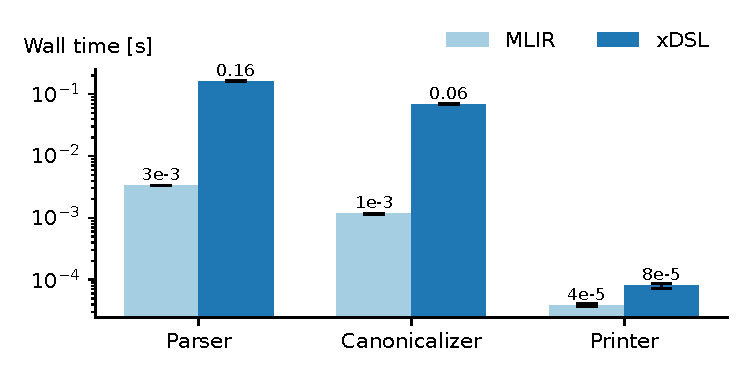
\includegraphics[width=\textwidth]{images/13_measuring_compiler_performance/walltimes.pdf}
        \caption{All pipeline phases of MLIR are faster than xDSL.}
        \label{fig:end-to-end-constant-folding-walltime}
    \end{subfigure}
    \hfill
    \begin{subfigure}[b]{0.45\textwidth}
        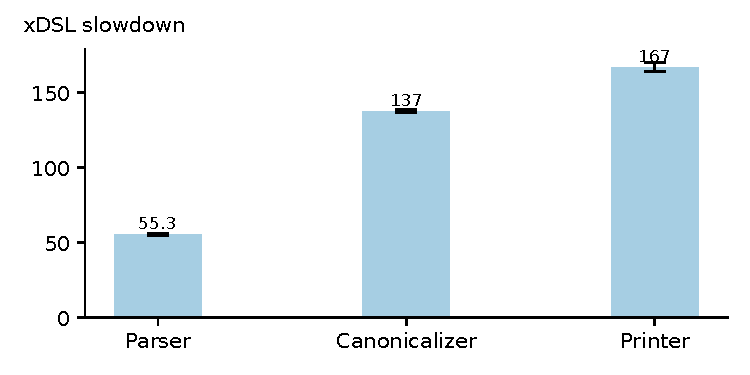
\includegraphics[width=\textwidth]{images/13_measuring_compiler_performance/speedup.pdf}
        \caption{.}
        \label{fig:end-to-end-constant-folding-speedup}
    \end{subfigure}
    \caption{.}
    \label{fig:end-to-end-constant-folding}
\end{figure}


%% Discuss results
% Hook
Despite its simplicity, this initial experiment reveals a number of interesting insights.
% Argument
Firstly, the current version of MLIR is much more performant than xDSL, with the pipeline phases having at best a $55\times$ slowdown, and at worst a $167\times$ slowdown.
Secondly, different pipeline phases constitute different proportions of the workloads, with the parser dominating both the xDSL and MLIR implementations runtime.
This motivates examining the parser as low-hanging fruit for optimisation, as by Amdahl's law, improving it by a fixed proportion would result in the greatest runtime reduction than any other pipeline phase.
However, this line of reasoning has two flaws. Firstly, the parser is disproportionately represented in constant folding workloads, which have few optimisation passes and very small outputted \acs{ir}. Secondly, it has the smallest slowdown of the pipeline phases (\autoref{fig:end-to-end-constant-folding-speedup}), suggesting other phases may have more opportunities for optimisation before being bounded by properties of the language runtime.
% Link
As such, we select the pattern rewriting phase, which implements the canonicalizer, for optimisation. This choice is motivated by its moderate contribution to runtime and slowdown over MLIR, combined with the technical interest of optimisation logic over parsing or printing.

%% Discuss why to pick pattern rewriter

% TODO: Parser/printer is for debug purposes, its not actually used in the real world for like nn tasks







% TODO: Do we even need this section? What does it add -- nothing since repeats less well what we do in specialisation. Just need to segue effectively to micro-benchmarks

% \section{Pattern rewriting}
% %% Introduction
% % Hook
% Having selected pattern rewriting as the compilation phase to examine in detail, we can modify our benchmarks to drive only
% % Figure: MLIR vs xDSL scaling across workloads?
% % Figure: Trace of MLIR and xDSL overall?








\section{Micro-benchmarks}
\label{sec:ubenchmark}

% Hook
Micro-benchmarking refers measuring the performance of fast, granular, and isolated segments of code.
% Argument
The term was coined by Saavedra et al. in their 1995 paper \cite{saavedraPerformanceCharacterizationOptimizing1995} ``Performance Characterization of Optimizing Compilers''. As such, we are in good company in our application of micro-benchmarking approaches to this problem domain.
Micro-benchmarks have many desirable properties. Since they run quickly, they can cheaply be repeated for statistical confidence.
Furthermore, their fine granularity makes them tractable to reason about -- providing useful information to optimise the component of the system they measure.
However, a key difficulty of micro-benchmarking is ensuring alignment with overall system performance. For example, the selection of code paths to micro-benchmark may introduce bias, making them less representative of the overall system. In addition to this, their performance may be inflated as a consequence of warmed caches and JIT optimisations across repeats, which would not occur during normal operation.
% Link
As such, micro-benchmarking is a useful tool for deeply understanding the performance of software, but must be used carefully to ensure the validity of its results.

% Hook
As discussed in our related work (Section \ref{sec:perf-user-extensible-frameworks}), Amini and Nui's talk ``How Slow is MLIR'' \cite{aminiHowSlowMLIR2024} discusses a set of micro-benchmarks for key operations in the MLIR compiler, such as traversing the IR and creating operations.
% Argument
These micro-benchmarks were used to inform the optimisation of MLIR's data structures and for comparison with traditional LLVM-based compilers. The implementation of the micro-benchmarks allude to an underlying design goal in MLIR by their measurement of asymptotic scaling properties\footnote{\url{https://github.com/joker-eph/llvm-project/blob/6773f827b9ee8055063fcf6b2c6fcdc7f4f579d2/mlir/unittests/Benchmarks/Cloning.cpp\#L66}}. This design goal is asymptotically optimal performance for its underlying data structures. However, data structures with these characteristics often incur constant-time penalties.
This causes overhead for small workloads, where, unlike the asymptotic case, the cost is not amortised. As such, micro-benchmarks may not be representative of the system's overall performance, revealing possibility for the optimisation of code co-designed using them.
Despite this, they can still provide useful insight into MLIR's performance characteristics.
% Link
We implement micro-benchmark workloads for the xDSL equivalent to those for MLIR presented in the keynote, and compare the results of these benchmarks between the two implementations, giving insights into their relative performance.
% We further leverage profiling tools to examine the execution of the two implementations. This allows us to distinguish the cost incurred by the language runtime from the cost incurred by the algorithmic approach of the implementation.

\subsection{Implementation}
\label{ssec:ubenchmark-implementation}

%% Finding and building the MLIR microbenchmarks
% Hook
Unfortunately, the implementation and build instructions for the ``How Slow is MLIR?'' micro-benchmarks were not published with the talk.
% Argument (too informal?)
However, their source code can be found on a branch of the presenter's fork of LLVM\footnote{\url{https://github.com/joker-eph/llvm-project/tree/benchmarks}}. We provide a copy of this source code and instructions for running the benchmarks\footnote{\url{https://github.com/EdmundGoodman/llvm-project-benchmarks}} to enhance the replicability of our results and facilitate further performance experiments.
% Link
This source code can then be used to construct comparable micro-benchmarks in Python.

%% Design of our microbenchmarks
% Hook
A key design goal of our micro-benchmarks for xDSL is parity with those provided for MLIR, ensuring the validity their direct comparison.
% Argument
As such, their implementation was derived from the MLIR benchmarks, matching test data and function invocations as closely as possible.
% Link
In the following sections, we discuss the implementations of a number of micro-benchmarks, facilitating discussion of the insights they give into compiler performance across implementations and language runtimes in later chapters.


%% Experimental procedure: Repeat 32768 times, and uncertainty as standard deviation
% Hook
Due to their inherently short length, we repeated meas
% Argument
% Link


\subsection{Operation trait checks}
\label{ssec:ubenchmark-trait-checks}

%% Micro-benchmark motivation and details
% Hook
MLIR and xDSL both provide methods to check whether operations have traits.
% Argument
These methods are used very frequently in common tasks. For example, when pattern rewriting over a block of IR, the traits of the block's constituent operations are often used by the matching engine to identify valid rewrites.

% There are two factors which contribute to this slow-down. The first is the inherent overhead incurred by the interpreter loop and data structures in Python's dynamic language runtime. The second is differences in implementation between xDSL and MLIR.
% % Link
% Examining this micro-benchmark in detail allows us to decouple the performance contributions of the implementation and language runtime, and provides insight into the impact of dynamism on user-extensible compiler framework workloads.

\begin{figure}[H]
    \centering
    \begin{subfigure}[b]{0.45\textwidth}
       \centering
        \begin{minted}[fontsize=\footnotesize]{c++}
            // Setup
            Operation op = b.create<OpWithRegion>(
                unknownLoc
            );

            // Benchmark
            bool hasTrait = op->hasTrait<
                OpTrait::SingleBlock
            >();
        \end{minted}
        \caption{``How Slow is MLIR?'' C++ implementation.}
        \label{listing:ubenchmark-trait-checks-bench-mlir}
    \end{subfigure}
    \hfill
    \begin{subfigure}[b]{0.45\textwidth}
        \centering
        \begin{minted}[breakanywhere,fontsize=\footnotesize]{python}
            # Setup
            op = OpWithRegion()

            # Benchmark
            has_trait = op.has_trait(SingleBlock)
        \end{minted}
        \footnotesize\vspace{2em}
        \caption{xDSL Python implementation.}
        \label{listing:ubenchmark-trait-checks-bench-xdsl}
    \end{subfigure}
    \vspace{1em}
    \captionsetup{name=Listing}
    \caption{Micro-benchmark implementations for methods checking an operation has a trait.}
    \label{listing:ubenchmark-trait-checks-bench}
\end{figure}

Micro-benchmarks of checking traits for both implementations (Listing \ref{listing:ubenchmark-trait-checks-bench}) show a slow-down of approximately $130\times$ from MLIR to xDSL (\autoref{tab:ubenchmark-trait-checks}).

\begin{table}[H]
  \caption{Trait checks in xDSL are approximately $130\times$ slower than in MLIR in the asymptotic case.} %, repeated ten times over $32768$ operations. Methodology is discussed in detail in Appendix \ref{} to facilitate replicability.}
  \label{tab:ubenchmark-trait-checks}
  \centering
  \begin{tabular}{cc}
    \toprule
    \textbf{MLIR [ns]} & \textbf{xDSL [ns]}\\
    \midrule
    $3.89 \pm 0.01$ & $504 \pm 76$ \\
    \bottomrule
  \end{tabular}
\end{table}


% % Hook
% The trait checking micro-benchmark yields two key insights.
% % Argument
% The first is that the original implementation of xDSL makes significant tradeoffs of performance for expressivity. By eliminating these tradeoffs, we reveal the Python language runtime incurs a $16\times$ overhead with respect to C++, as a result of the complexity of its evaluation loop.
% The second is that whilst C++ can efficiently represent dynamic functionality, albeit at the cost of implementation complexity, dynamism incurs the cost of obscuring other optimisations that would further widen the performance gap between Python and C++.
% % Link
% However, whilst trait checking is a frequent operation, it alone is not representative of the overall performance of compiler frameworks. As such, further micro-benchmarks and examining representative workloads is required.


\subsection{Operation instantiation}
\label{ssec:ubenchmark-operation-instantiation}

% Hook
Operations are a central data structure in MLIR and xDSL's \ac{ir} representation, constituting dialects and composing together into programs. As such, the methods to instantiate operations a very frequently invoked.
% Argument
% Link


\begin{table}[H]
  \caption{Operation instantiation in xDSL is approximately $xyz\times$ slower than in MLIR in the asymptotic case.} %, repeated ten times over $32768$ operations. Methodology is discussed in detail in Appendix \ref{} to facilitate replicability.}
  \label{tab:ubenchmark-trait-checks}
  \centering
  \begin{tabular}{cc}
    \toprule
    \textbf{MLIR [ns]} & \textbf{xDSL [ns]}\\
    \midrule
    $3.89 \pm 0.01$ & $504 \pm 76$ \\
    \bottomrule
  \end{tabular}
\end{table}



\subsection{Operation traversal}
\label{ssec:ubenchmark-operation-traversal}

% Hook
Operations are a central data structure in MLIR and xDSL's \ac{ir} representation, constituting dialects and composing together into programs. As such, the methods to instantiate operations a very frequently invoked.
% Argument
% Link


\subsection{Summary of micro-benchmarks}
% \label{ssec:ubenchmark-summary}


%% Perhaps don't talk about remaining ones so concretely? Could move stuff to appendix?
% Hook
% Argument
% Link




% % Hook
% In addition to the above micro-benchmarks which we examine in detail, we further provide a wider suite of micro-benchmarks discussed in lesser detail for brevity. % The implementations of all xDSL micro-benchmarks are provided in the Appendix (\autoref{}).
% % Argument
% This suite implements many of the remaining equivalent micro-benchmarks from ``How Slow is MLIR'' (\autoref{tab:ubenchmark-remaining-mlir}).
% From these, we can see the trend of a slow-down in the order of $xy\times$ holds

% \begin{table}[H]
%   \caption{.}
%   \label{tab:ubenchmark-remaining-mlir}
%   \centering
%   \begin{tabular}{ccc}
%     \toprule
%     \textbf{Benchmark name} & \textbf{MLIR [ns]} & \textbf{xDSL [ns]}\\
%     \midrule
%     Trait checks & $3.89 \pm 0.01$ & $504 \pm 76$ \\
%     ... & ... & ... \\
%     \bottomrule
%   \end{tabular}
% \end{table}


% % Hook
% In addition to the remaining ``How Slow is MLIR?'' micro-benchmarks, the suite provides further xDSL-only micro-benchmarks sampled from atomic functions invoked by pattern rewriting workloads. % (\autoref{tab:ubenchmark-xdsl-regression}).
% % Argument
% These have two-fold use: triaging functions to optimise by longest runtime following Amdhal's law \cite{amdahlValiditySingleProcessor1967}; and serving as a metric of performance to ensure optimisations don't inadvertently introduce regressions.
% % Link

% %% Do a bar chart instead of a table!!!!
% %% Might want table for raw values and bar chart of speedups? Very big differences don't plot neatly...
% % \begin{table}[H]
% %   \caption{.}
% %   \label{tab:ubenchmark-xdsl-regression}
% %   \centering
% %   \begin{tabular}{ccc}
% %     \toprule
% %     \textbf{Benchmark name} & \textbf{xDSL [ns]}\\
% %     \midrule
% %     Trait checks & $504 \pm 76$ \\
% %     ... & ... & ... \\
% %     \bottomrule
% %   \end{tabular}
% % \end{table}
